\documentclass{beamer}
\usetheme{CambridgeUS}

\setbeamertemplate{caption}[numbered]{}

\usepackage{amsmath}
\usepackage{amssymb}
\usepackage{gensymb}
\usepackage{graphicx}
\usepackage{txfonts}
\usepackage{circuitikz}
\def\inputGnumericTable{}

\usepackage[latin1]{inputenc}                                 
\usepackage{color}                                            
\usepackage{array}                                            
\usepackage{longtable}                                        
\usepackage{calc}                                             
\usepackage{multirow}                                         
\usepackage{hhline}                                           
\usepackage{ifthen}
\usepackage{caption} 
\captionsetup[table]{skip=3pt}

\providecommand{\pr}[1]{\ensuremath{\Pr\left(#1\right)}}
\providecommand{\brak}[1]{\ensuremath{\left(#1\right)}}
\providecommand{\cbrak}[1]{\ensuremath{\left\{#1\right\}}}

\renewcommand{\thefigure}{\arabic{table}}
\renewcommand{\thetable}{\arabic{table}}                                     
                               
\title{EE3900:Linear Systems and Signal Processing}
\subtitle{Lab Report}
\author{Lokesh Badisa \\ AI21BTECH11005}
\date{Nov 2022}


\begin{document}
	% The title page
	\begin{frame}
		\titlepage
	\end{frame}
	
	% The table of contents
	\begin{frame}{Outline}
    		\tableofcontents
	\end{frame}
\section{Cover Page}
\begin{frame}{Cover}
	\begin{itemize}
		\item Title: Working Model of Mobile Charger
		\item Date: 4-5 Segment of $3^{rd}$ segment
		\item Team/Individual Project: Individual Project
		\item Course: EE3900
	\end{itemize}
\end{frame}
\section{Apparatus}
\begin{frame}
	\begin{itemize}
		\item BreadBoard or PCB
		\item Transformer(12V-0-12V)
		\item 7805 Regulator
		\item Diodes(4)
		\item 100$\micro$F Capacitor
		\item Connecting Wires
		\item Soldering Equipment
	\end{itemize}
\end{frame}
\section{Circuit Diagram}
\begin{frame}{Circuit Diagram}
\begin{circuitikz}[american]
\draw (0,0) node [transformer](T){};
\draw (T.B1) to ++(4,0)
to ++(0,-0.5) to [D] ++(2,0)
to ++(0,-1) to  [D,invert] ++(-2,0)
to [D,invert] ++(-2,0) to ++(0,1)
to [D] ++(2,0);
\draw (T.B2) to ++(4,0);
\draw (3,0) to ++(-0.5,0)
to ++(0,-2) to ++(7.5,0) to ++(0,3);
\draw (8.5,-2) to [C,l=$100\mu F$]++(0,2) to ++(-1.5,0);
\draw (8.5,0) to ++(1,0) to ++(0,1) to ++(-0.5,0)
to ++(0,0.75) to ++(2,0) to ++(0,-0.75) to [short,l_=$7805$]++(-1.5,0);
\draw (5,-0.45) to ++(0,-0.59);
\draw (10.5,1) to ++(0,-1) to ++(1,0);
\draw(T.A1) to[open,v<={$240V_{rms}$}](T.A2);
\draw(T.B2) to[open,v>=$12V_{rms}$](T.B1);
\end{circuitikz}
\end{frame}
\section{Waveforms}
\begin{frame}{Input Waveforms:18V Peak}
\begin{figure}[!ht]
    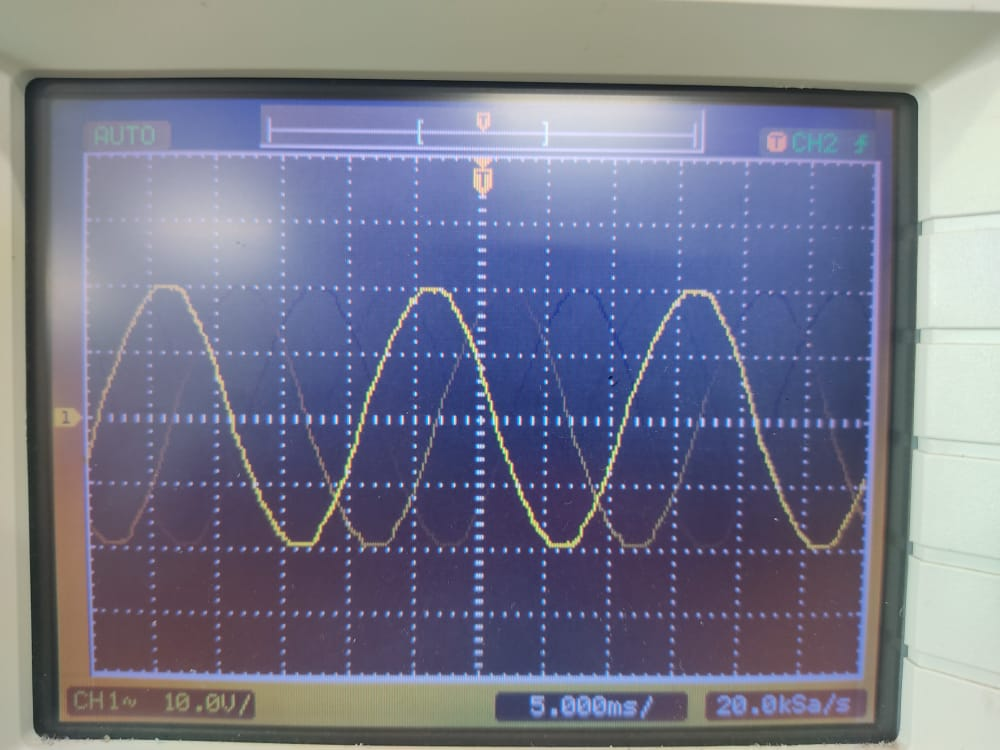
\includegraphics[width=\columnwidth]{figs/input.jpeg}
    \caption{Output AC waveform at transformer stage across T\textsubscript{1}T\textsubscript{0} (18 V peak).}
    \label{fig:transformer}
\end{figure}
\end{frame}
\begin{frame}{Output Waveform:Constant 5V}
\begin{figure}[!ht]
    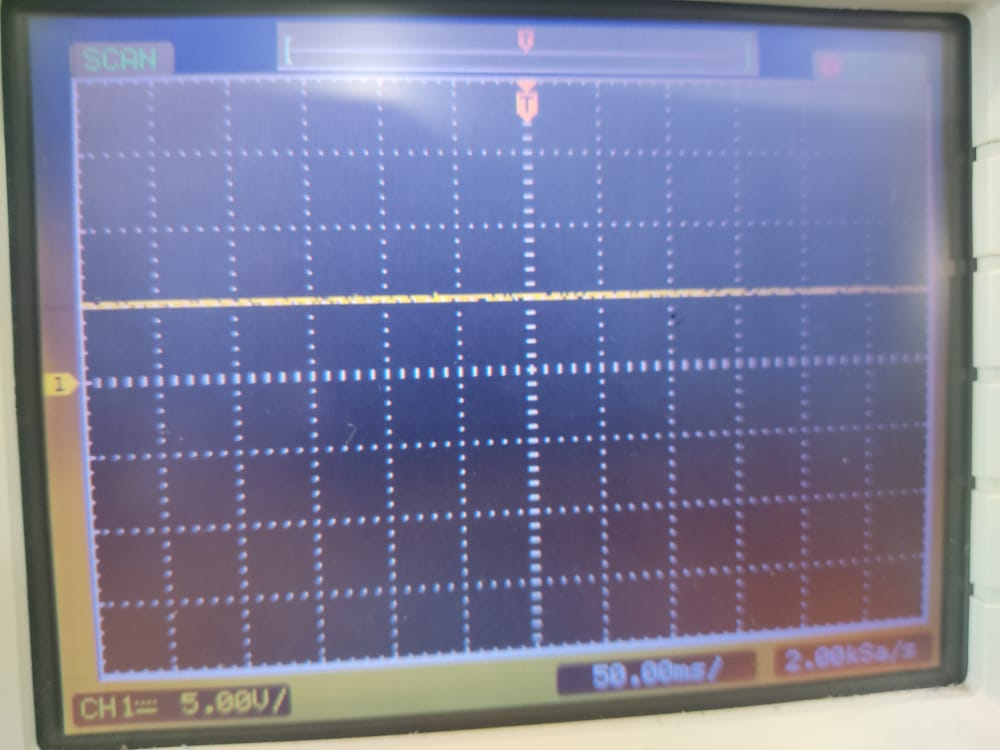
\includegraphics[width=\columnwidth]{figs/output.jpeg}
	\caption{Output Waveform for Charging(Constant 5V)}
    \label{fig:transformer}
\end{figure}
\end{frame}
\begin{frame}{Half-Wave Rectified Waveform:Peak 18V}
	\begin{figure}[!ht]
		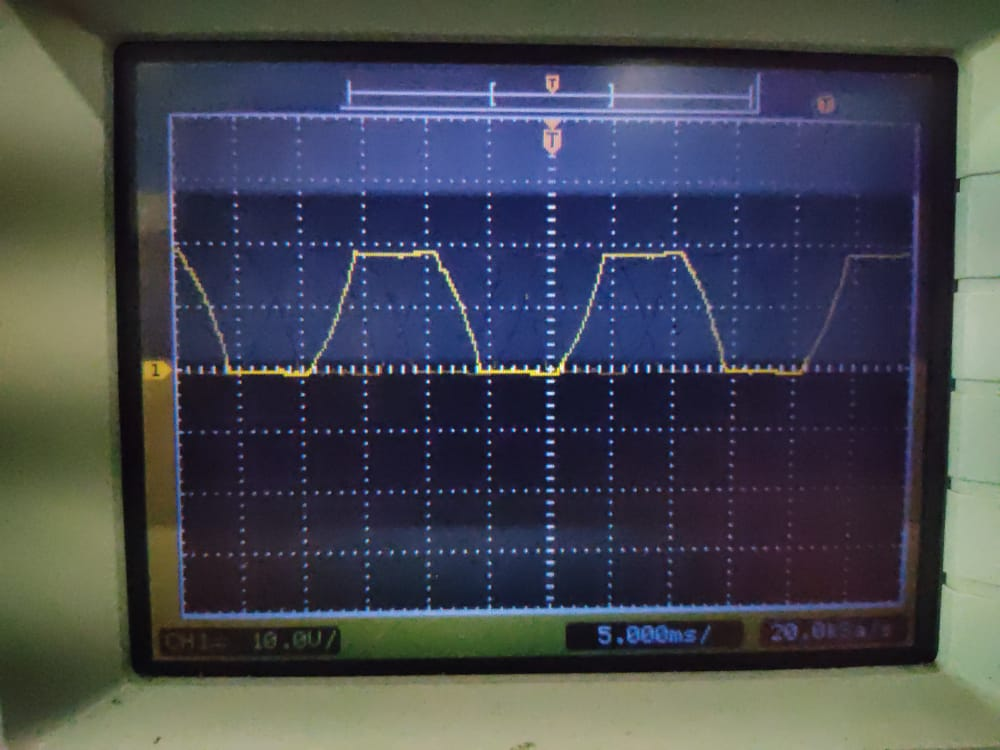
\includegraphics[width=\columnwidth]{figs/rectifiedwave.jpeg}
	\end{figure}
\end{frame}
\begin{frame}{Output DC Waveform at Filter Stage:Constant 18V}
	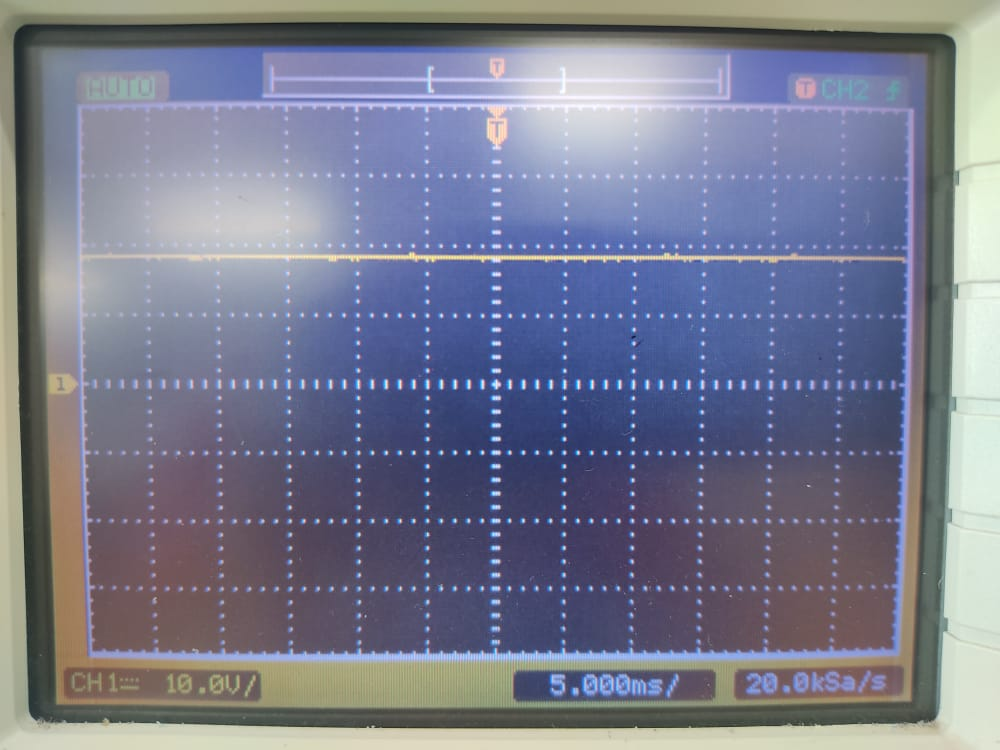
\includegraphics[width=\columnwidth]{figs/3.jpeg}
\end{frame}
\end{document}
